\documentclass[a4paper, 11pt]{exam}
\usepackage{titling}
\newcommand{\subtitle}[1]{%
  \posttitle{%
    \par\end{center}
    \begin{center}\large#1\end{center}
    }%
}

\usepackage{url}
\usepackage{amsmath,amsthm,enumitem,amssymb}
\usepackage{graphicx}
\usepackage{hyperref}
\renewcommand{\labelenumii}{\roman{enumii}}

\title{Homework Assignment 2}
\subtitle{CS/ECE 6810: Computer Architecture \\
September 26,2018
\\
Name: Jake Pitkin

UID: u0891770 }

\author{ \\
\textbf{ILP and Branch Prediction}}
\date{Due Date: October 03, 2018.\\
120 points}

\begin{document}
\maketitle
\begin{center}

\begin{enumerate}
	
\item \textbf{Multi-cycle Instructions.}
A pipelined architecture comprises instruction fetch (IF), instruction decode (ID), register read (RR), execute (EX), and write-back (WB) stages.
\begin{figure}[!h]
	\centering
	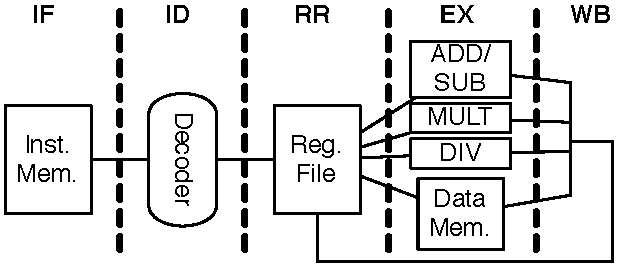
\includegraphics[width=0.5\linewidth]{q1}
	\caption{Pipelined core architecture.}
	\label{fig:q1}
\end{figure}

Except EX, each stage requires one clock cycle to complete.
The EX stage includes 4 functional units that perform memory and ALU operations---e.g., ADD, SUB, MULT, DIV, load, and store.
The table below shows the latency of each operation in terms of clock cycles.
The architecture implements forwarding paths from the EX/WB pipeline registers to the EX input.
Moreover, the register file may be bypassed during the WB stage to send the register value to EX.

\begin{center}
\begin{tabular}{ |c|c|c|c|c|c|c| } 
 \hline
  & ADD & SUB & MULT & DIV & Load & Store \\ 
  \hline
 Latency & 1 & 1 & 3 & 7 & 2 & 1 \\ 
 \hline
\end{tabular}
\end{center}

\begin{enumerate}
\item Identify all structural and data hazards in the following code. \textbf {(10 points)}

%\newline

\begin {center}
Load F6, 20(R5) 

Load F2, 28(R5)

MUL F0, F2, F4

SUB F8, F6, F3

DIV F10, F0, F6

ADD F6, F8, F2

Store F8, 50(R5)

\end {center}

\hfill
 
\textbf{Answer:} Below is a table of all structural and data hazards present in the above list of instructions. \textit{Instruction 1} is the instruction that comes first temporally which is followed by \textit{Instruction 2}. \textit{Hazard Type} indicates what type of hazard is detected and \textit{Register} is the register causing the hazard.

\begin{center}
\begin{tabular}{ |c|c|c|c| } 
 \hline
  \textbf{Instruction 1} & \textbf{Instruction 2} & \textbf{Hazard Type} & \textbf{Register} \\ 
  \hline
 Load F2, 28(R5) & MUL F0, F2, F4 & RAW & F2\\ \hline
 Load F6, 20(R5) & SUB F8, F6, F3 & & F6\\ \hline
 MUL F0, F2, F4 & DIV F10, F0, F6 &  & F0 \\ \hline
 Load F6, 20(R5) & DIV F10, F0, F6 &  & F6 \\ \hline
 SUB F8, F6, F3 & ADD F6, F8, F2 & & F8\\ \hline
 Load F2, 28(R5) & ADD F6, F8, F2 & & F2\\ \hline
\end{tabular}
\end{center}

\hfill

\pagebreak
\item Create a timing diagram for the code showing the execution of the code in time (clock cycles). \textbf{(20 points)}

\begin{center}
\begin{tabular}{ |c|c|c|c|c|c|c| } 
 \hline
  \textbf{Instruction} & \textbf{Cycle 1} & \textbf{Cycle 2} & \textbf{Cycle 3} & \textbf{Cycle 4} & \textbf{Cycle 5} & 
  \textbf{Cycle 6 \ \ \ \ \ \ \ \ \ \ } \\ 
  \hline
 Load F6, 20(R5) & IF & ID & RR & EX Data & EX Data & WB\\ \hline
 Load F2, 28(R5) & - & IF & ID & RR & STALL & EX Data\\ \hline
 MUL F0, F2, F4 & - & - & IF & ID & RR & STALL\\ \hline
 SUB F8, F6, F3 & - & - & - & IF & ID & RR\\ \hline
 DIV F10, F0, F6 & - & - & - & - & IF & ID\\ \hline
 ADD F6, F8, F2 & - & - & - & - & - & IF\\ \hline
 Store F8, 50(R5) & - & - & - & - & - & -\\ \hline
\end{tabular}

\begin{tabular}{ |c|c|c|c|c|c|c| } 
 \hline
  \textbf{Instruction} & \textbf{Cycle 07} & \textbf{Cycle 08} & \textbf{Cycle 09} & \textbf{Cycle 10} & \textbf{Cycle 11} & 
  \textbf{Cycle 12} \\ 
  \hline
 Load F6, 20(R5) &  &  &  &  &  & \\ \hline
 Load F2, 28(R5) & EX Data & WB &  &  &  & \\ \hline
 MUL F0, F2, F4 & STALL & EX MULT & EX MULT & EX MULT & WB &\\ \hline
 SUB F8, F6, F3 & EX SUB & STALL & STALL & STALL & STALL & WB\\ \hline
 DIV F10, F0, F6 & RR & STALL & STALL & STALL & EX DIV & EX DIV\\ \hline
 ADD F6, F8, F2 & ID & RR & EX ADD & STALL & STALL & STALL\\ \hline
 Store F8, 50(R5) & IF & ID & RR & EX Data & STALL & STALL\\ \hline
\end{tabular}

\begin{tabular}{ |c|c|c|c|c|c|c| } 
 \hline
  \textbf{Instruction} & \textbf{Cycle 13} & \textbf{Cycle 14} & \textbf{Cycle 15} & \textbf{Cycle 16} & \textbf{Cycle 17} & 
  \textbf{Cycle 18 \ \ } \\ 
  \hline
 Load F6, 20(R5) &  &  &  &  &  & \\ \hline
 Load F2, 28(R5) &  &  &  &  &  & \\ \hline
 MUL F0, F2, F4 &  &  &  &  &  & \\ \hline
 SUB F8, F6, F3 &  &  &  &  & & \\ \hline
 DIV F10, F0, F6 & EX DIV & EX DIV & EX DIV & EX DIV & EX DIV & WB\\ \hline
 ADD F6, F8, F2 & STALL & STALL & STALL & STALL & STALL & STALL\\ \hline
 Store F8, 50(R5) & STALL & STALL & STALL & STALL & STALL & STALL\\ \hline
\end{tabular}

\begin{tabular}{ |c|c|c|c|c|c|c| } 
 \hline
  \textbf{Instruction} & \textbf{Cycle 19} & \textbf{Cycle 20} & \textbf{Cycle 21} & \textbf{Cycle 22} & \textbf{Cycle 23} & 
  \textbf{Cycle 24 \ \ } \\ 
  \hline
 Load F6, 20(R5) &  &  &  &  &  & \\ \hline
 Load F2, 28(R5) &  &  &  &  &  & \\ \hline
 MUL F0, F2, F4 &  &  &  &  &  & \\ \hline
 SUB F8, F6, F3 &  &  &  &  &  & \\ \hline
 DIV F10, F0, F6 &  &  &  &  &  & \\ \hline
 ADD F6, F8, F2 & WB &  &  &  &  & \\ \hline
 Store F8, 50(R5) & STALL & WB &  &  &  & \\ \hline
\end{tabular}
\end{center}


\end{enumerate}
\textbf{My Notes for the above timelne:}
%
\begin{itemize}
	\item Stalls are used to maintain the WB order of the instructions even if there is no hazard.
	\item Instruction MUL F0, F2, F4 will have its register read of F2 overwritten in cycle 8 by a forward from the EX/WB pipeline. 
	\item Instruction ADD F6, F8, F2 will have it's register read of F8 overwritten in cycle 9 by a forward from the EX/WB pipeline.
	\item Instruction Store F8, 50(R5) will have its register read of F8 overwritten in cycle 10 by a forward from the EX/WB pipeline.
	\item Instruction DIV F10, F0, F6 will have its register read of F0 overwritten in cycle 11 by a forward from the EX/WB pipeline.

\end{itemize}

\pagebreak

\item \textbf{Points of Production and Consumption.}
Consider an unpipelined processor where it takes 36 ns to go through the circuits and 0.5 ns for the latch overhead. Assume that the point of production and point of consumption in the unpipelined processor are separated by 12ns. Assume that half the instructions do not introduce a data hazard and half the instructions depend on their preceding instruction.

\begin{enumerate}
\item What is the maximum throughput of the unpipelined architecture in instructions per second (IPS). \textbf{(10 points)} \\

\hfill
 
\textbf{Answer:} 

\hfill

\item We build a 12-stage pipelined architecture for the processor. Please compute the percentages of increase/decrease in throughput for the pipelined architecture compared to unpipelined process.\textbf {(10 points)}

\hfill
 
\textbf{Answer:} 

\hfill

\end{enumerate}
%\end{enumerate}

%\begin{enumerate}

\item \textbf {Software Optimization.}
Below are examples of a C and assembly codes for a \textbf{for}-loop.
Notice that \texttt{i} is an 8-byte long integer. Register names indicate if floating point (F) or integer (R) operations are necessary for instructions.

\begin{tabular}{lll}
	\textbf{Source code} & & \textbf{Assembly code }\\
	\texttt{for (i = 125; i > 0; i--) \{}&  &\hspace{40pt}\texttt{ADDI R1, R0, \#1000} \\
	\hspace{20pt}\texttt{x[i] = s * y[i] + z;} &  &\hspace{40pt}\texttt{JMP Chck}\\
	\texttt{\}} &  &\texttt{Loop: Load F1, 0(R1)} \\
    &  &\hspace{35pt}\texttt{ MUL F3, F1, F2}\\
	&  &\hspace{35pt}\texttt{ ADD F5, F3, F4}\\
	&  &\hspace{35pt}\texttt{ Store F5, 20000(R1)}\\
	&  &\hspace{35pt}\texttt{ ADDI R1, R1, \#-8}\\
%	&  &\hspace{35pt}\texttt{ ADDUI R2, R2, \#-8}\\
	&  &\texttt{Chck: BNEQ R1, R0, Loop}\\
%	&  &\hspace{35pt}\texttt{ NOP}\\
\end{tabular}

Consider a five-stage scalar pipeline with multi-cycle functional units for floating-point and integer operations at the EX stage.
Assume the following delays between dependent (producer-consumer) instructions:\\
(a) Load feeding any instruction: 1 stall cycle\\
(b) FP MULT/ADD feeding store: 4 stall cycles\\
(c) Integer ADD feeding a branch: 1 stall cycle\\
(d) A conditional branch has 1 delay slot (the next instruction after a conditional branch is fetched and executed to completion without knowing the outcome of the branch)

\begin{enumerate}
	\item First show all of the stall cycles necessary in the original assembly code. Then, find an optimized schedule for this loop through reordering instructions but \underline{without} resorting to loop \underline{unrolling.} \textbf{(10 points)}
	
	\hfill
 
\textbf{Answer:} 

\hfill
	
	\item Optimize the schedule by loop unrolling 1x, 2x, and 3x. Notice that a 1x unroll includes the original loop body plus the 1 time unrolled instructions. \textbf{(10 points)}
	
	\hfill
 
\textbf{Answer:} 

\hfill


\end{enumerate}
%Note: Assume that if all existing separate pipes at the same time are idle then there would be a stall.
%\end{enumerate}



%\item \textbf{Impact of Microarchitectural Techniques.}
%Consider a multiple-issue archiecture with the latency mentioned in the following table. Suppose you have two execution pipelines, each capable of beginning execution of one instruction per cycle, and enough fetch/decode bandwidth in the front end so that it will not stall your execution. In addition, assume results can be immediately forwarded from one execution unit to another, or to itself. Further, assume that the only reason an execution pipeline would stall is due to true data dependency. 
%\begin{center}
%	\begin{tabular}{ |c|c|c|c|c|c|c|c| } 
%		\hline
%		& MemLD & MemSD & Integer ADD,SUB & Branch & ADDD & MultD & DIVD \\ 
%		\hline
%		Latency & 3 & 1 & 0 & 1& 2 & 4 & 10 \\ 
%		\hline
%	\end{tabular}
%\end{center}
%
%\begin {center}
%\hspace{-20pt} Loop: LD  F2, 0(Rx) 
%
%\hspace{25pt} MULTD F2, F0, F2
%
%\hspace{15pt} DIVD  F8, F2, F0
%
%\hspace{0pt} LD F4, 0(RY)
%
%\hspace{20pt} ADDD F4, F0, F4
%
%\hspace{24pt} ADDD F10, F8, F2
%
%\hspace{1pt} SD  F4, 0(RY)
%
%\hspace{20pt} ADDI Rx, Rx, \#8
%
%\hspace{20pt} ADDI Ry, Ry, \#8
%
%\hspace{20pt} SUB  R20, R4, Rx
%
%\hspace{10pt} BNZ  R20, Loop
%
%\end {center}
%
%\begin{enumerate}
%	\item How many cycles per loop does the above code require to execute? \textbf{(15 points)}
%	
%	\item In the above multiple-issue design, you may have recognized some subtle issues.For example, if instruction N  begins execution in Execution Pipe 0 at the same time that instruction N+1 begins in Pipe 1, and N + 1 requires a shorter execution latency than N, then N + 1 will complete before N (even though program ordering would have implied otherwise). Mention at least two reasons why that could be hazardous and will require special considerations in the microarchitecture. Give an example of two instructions from the code that demonstrate this hazard? \textbf {(15 points)}
%	
%	
%	
%\end{enumerate}


\item \textbf{Branch Prediction.}
Assume a 32-bit five-stage scalar pipeline with the fetch, decode, execute, memory, and write back stages.
All pipeline stages require 1 cycle except the load and store operations that need 3 cycles to access the data memory; branch instructions need 2 clock cycles to determine the outcome.
Example C and assembly codes are given for a user application.

\begin{tabular}{lll}
	\textbf{Source code} & & \textbf{Assembly code }\\
	\texttt{n = 250;}&  &\hspace{40pt}\texttt{ADDI R3, R0, \#1000} \\
	\texttt{i = 0;} &  &\hspace{40pt}\texttt{ADDI R2, R0, \#0}\\
	\texttt{do \{} &  &\texttt{Loop: Load  R1, 0(R2)} \\
	\hspace{20pt}\texttt{x[i] = x[i] + 1;}&  &\hspace{40pt}\texttt{ADDI   R1, R1, \#1}\\
	\hspace{20pt}\texttt{i = i+1;}&  &\hspace{40pt}\texttt{Store  R1, 0(R2)}\\
	\texttt{\} while(i < n);}&  &\hspace{40pt}\texttt{ADDI R2, R2, \#4}\\
	&  &\hspace{40pt}\texttt{SUB R4, R3, R2}\\
	&  &\hspace{40pt}\texttt{BNEQ R4, R0, Loop}\\
\end{tabular}

%There is no forwarding. Show the phases of each instruction per clock cycle for one iteration of the loop.
\begin{enumerate}
	\item  Without any branch prediction, how many stall cycles are necessary due to the branch instructions in the original code? \textbf {(10 points)}
	
\hfill
 
\textbf{Answer:} 

\hfill

    \item  Assume a static branch predictor capable of predicting always-taken or always-not-taken. Compute the percentages of improvements in IPC compared to the previous case with no branch predictor? \textbf {(10 points)}
    
    \hfill
 
\textbf{Answer:} 

\hfill

   \item Assume a single 3-bit saturating counter for dynamic branch prediction. The initial state of the counter is 000. States 000--011 predict not taken; while, 100--111 indicate taken. Compute the total number of mis-predictions. Compute the percentages of improvements in IPC compared to the case with no branch predictor? \textbf {(10 points)}
   
   \hfill
 
\textbf{Answer:} 

\hfill

\end{enumerate}
Note: Assume an instruction does not enter the execution phase until all of its operands are ready.



\item \textbf{Bonus Question.}
Consider running the following code on a pipelined machine. Every pipeline stage requires one cycle. Every branch instruction needs three cycles to produce an outcome. Assume that only branches may introduce stall cycles to the pipeline.
We want to design a global branch predictor with 32 2-bit counters (n=2), where 5 bits from the PC are XORed with a 5-bit GHR (b=r=5) to produce an index to the shared counters.
\begin{enumerate}
	\item  Without any branch prediction, compute the IPC of the code? \textbf {(5 points)}
	\item  Assume all the shared counters and the GHR are initialized to 0, compute the IPC and misprediction rate of the global branch predictor? \textbf{(15 points)}
\end{enumerate}
Note: after executing a branch, GHR shifts 1 bit to the left. The least significant bit of GHR is set to the branch outcome (0: not-taken and 1: taken).

\begin{figure}[!h]
	\centering
	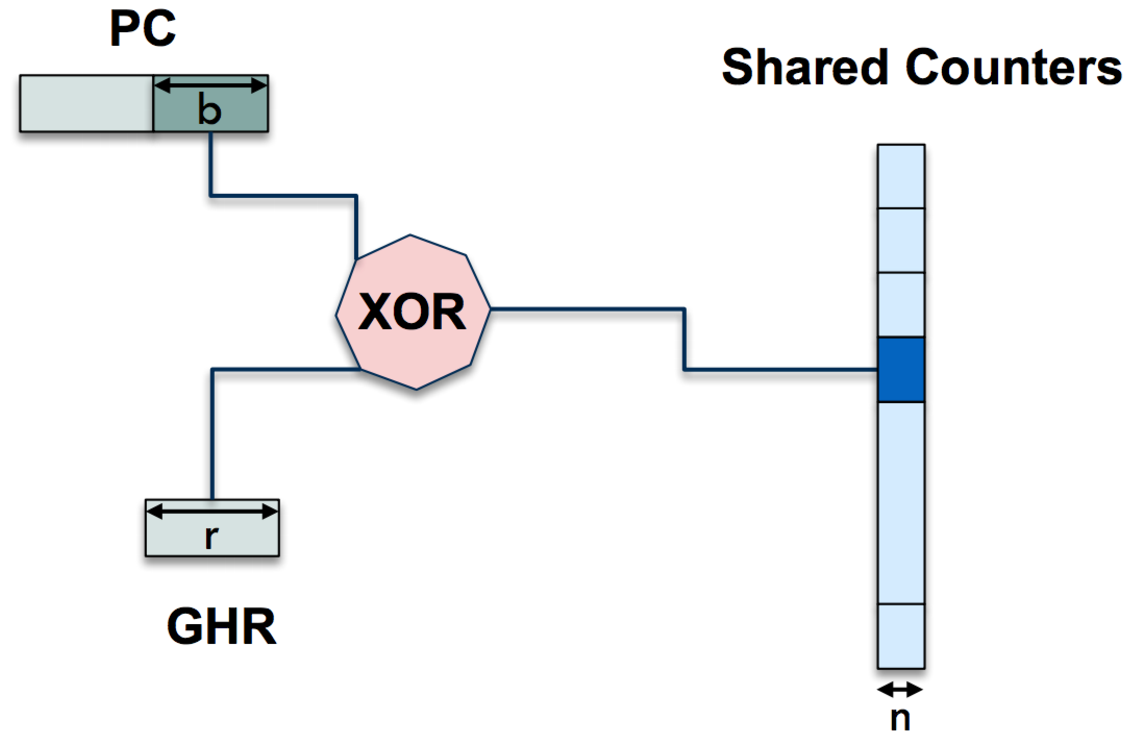
\includegraphics[width=0.5\linewidth]{q5}
	\caption{Global branch predictor.}
	\label{fig:q5}
\end{figure}


\begin{tabular}{lcl}
\textbf{PC} & : & \textbf{Instruction}\\
\hline
\texttt{0000} & : & \hspace{40pt}\texttt{ADDI R1, R0, \#1}\\
\texttt{0004} & : & \hspace{40pt}\texttt{ADDI R2, R0, \#9}\\
\texttt{0008} & : & \texttt{Loop: ADDI R2, R2, \#-1}\\
\texttt{0012} & : & \hspace{40pt}\texttt{ANDI R3, R2, \#3}\\
\texttt{0016} & : & \hspace{40pt}\texttt{BNEQ R3, R1, Next}\\
\texttt{0020} & : & \hspace{40pt}\texttt{ADD R4, R4, R3}\\
\texttt{0024} & : & \texttt{Next: BNEQ R2, R0, Loop}
\end{tabular}

\end{enumerate}


\end{document}